% Copyright 2004 by Till Tantau <tantau@users.sourceforge.net>.
%
% In principle, this file can be redistributed and/or modified under
% the terms of the GNU Public License, version 2.
%
% However, this file is supposed to be a template to be modified
% for your own needs. For this reason, if you use this file as a
% template and not specifically distribute it as part of a another
% package/program, I grant the extra permission to freely copy and
% modify this file as you see fit and even to delete this copyright
% notice. 

\documentclass{beamer}
\setbeamertemplate{navigation symbols}{}
%\useoutertheme{shadow}
\setbeamertemplate{headline}{}

\usepackage{amssymb}
\usepackage{amsthm}
\usepackage{amstext}
\usepackage{amsbsy}
\usepackage{amscd}
\usepackage{enumerate}
\usepackage{chngpage}
\usepackage{mathtools}
\usepackage{amsmath}
\usepackage{hyperref}
%\usepackage{enumitem}
%\usepackage{stmaryrd}
\usepackage{color}
\usepackage{wrapfig}

\theoremstyle{plain}


\newtheorem{alg}{Algorithm}
\newtheorem{thm}{Theorem}[section]
\newtheorem{lem}[thm]{Lemma} 
\newtheorem{cor}[thm]{Corollary}
\newtheorem{prop}[thm]{Proposition}
\theoremstyle{definition}
\newtheorem{defn}[thm]{Definition}
\newtheorem{question}[thm]{Question}
\newtheorem{conj}[thm]{Conjecture}
\newtheorem{obs}[thm]{Observation}
\newtheorem{claim}[thm]{Claim}
\newtheorem{rmk}[thm]{Remark}

\newcommand{\Z}{\mathbb Z}
\newcommand{\N}{\mathbb N}
\newcommand{\R}{\mathbb R}
\newcommand{\C}{\mathbb C}
\newcommand{\Q}{\mathbb Q}
\newcommand{\F}{\mathbb F}
\newcommand{\Fp}{\mathbb{F}_p}
\newcommand{\Fq}{\mathbb{F}_q}

\newcommand{\sthat}{\,|\,}
\newcommand{\stp}[1]{\st\left(#1\right)}

\newcommand{\hal}[1]{\mathrm{hal}(#1)}
\newcommand{\gal}[1]{\mathrm{gal}(#1)}

\newcommand{\reals}{\mathbb{R}}
\newcommand{\hreals}{\prescript{*}{}{\mathbb{R}}}
\newcommand{\nats}{\mathbb{N}}
\newcommand{\hnats}{\prescript{*}{}{\mathbb{N}}}

\newcommand{\hr}[1]{\prescript{*}{}{#1}}

\newcommand{\del}{\partial}

\DeclareMathOperator{\dom}{dom}
\DeclareMathOperator{\st}{st}
\DeclareMathOperator{\inx}{inx}

\usepackage{biblatex}
\addbibresource{Thesis_Bibliography.bib}

\usepackage{graphicx}
\graphicspath{ {./images/}}
\usepackage{subcaption}


% There are many different themes available for Beamer. A comprehensive
% list with examples is given here:
% http://deic.uab.es/~iblanes/beamer_gallery/index_by_theme.html
% You can uncomment the themes below if you would like to use a different
% one:
%\usetheme{AnnArbor}
%\usetheme{Antibes}
%\usetheme{Bergen}
%\usetheme{Berkeley}
%\usetheme{Berlin}
%\usetheme{Boadilla}
\usetheme{boxes}
%\usetheme{CambridgeUS}
%\usetheme{Copenhagen}
%\usetheme{Darmstadt}
%\usetheme{default}
%\usetheme{Frankfurt}
%\usetheme{Goettingen}
%\usetheme{Hannover}
%\usetheme{Ilmenau}
%\usetheme{JuanLesPins}
%\usetheme{Luebeck}
%\usetheme{Madrid}
%\usetheme{Malmoe}
%\usetheme{Marburg}
%\usetheme{Montpellier}
%\usetheme{Metropolis}
%\usetheme{PaloAlto}
%\usetheme{Pittsburgh}
%\usetheme{Rochester}
%\usetheme{Singapore}
%\usetheme{Szeged}
%\usetheme{Warsaw}

%\usecolortheme{albatross}
%\usecolortheme{beetle}
%\usecolortheme{crane}
%\usecolortheme{dove}
%\usecolortheme{fly}
%\usecolortheme{seagull}
%\usecolortheme{wolverine}
%\usecolortheme{beaver}
%\usecolortheme{lily}
%\usecolortheme{orchid}
%\usecolortheme{rose}
%\usecolortheme{whale}
\usecolortheme{seahorse}
%\usecolortheme{dolphin}

%%%SPACING
%\let\olditem\item
%\renewcommand{\item}{\setlength{\itemsep}{\fill}\olditem}

%\useoutertheme{split}
%\setbeamertemplate{navigation symbols}{}

\makeatletter
\setbeamertemplate{footline}{}

\makeatother
\usepackage{booktabs}
\usepackage{xcolor}
\usepackage{tikz}
\usetikzlibrary{calc}

\definecolor{purple}{RGB}{155, 13, 184}
\definecolor{pink}{RGB}{252, 53, 213}
\definecolor{teal}{RGB}{4, 189, 191}

\newcommand\zp{\normalfont{\raisebox{.5pt}{\textcircled{\raisebox{-.9pt} {z}}}}}
\newcommand\rp{\normalfont{\raisebox{.5pt}{\textcircled{\raisebox{-.9pt} {r}}}}}
\newcommand\rpp{\normalfont{\raisebox{.5pt}{\textcircled{\raisebox{-.9pt} {r'}}}}}

\definecolor{myGreen}{rgb}{0.09, 0.45, 0.27}
%\usecolortheme[named=myGreen]{structure}

%you can put the title, author, and date here
\title{Infinitesimal Calculus}

\author{Paul Schulze}

\date{}

%you always need to begin with this
\begin{document}
	
%this creates the title page
\begin{frame}
	\titlepage
\end{frame}
	
%\begin{frame} creates a slide. You put the slide title in {} directly after \begin{frame}.

\begin{frame}{History}
\begin{itemize}
	\item Newton \& Leibniz formulated calculus using the idea of \textit{infinitesimals}
	\item Infinitesimals are really really small, but not $0$
	\item Considered nonsensical, replaced with $\delta$-$\epsilon$
	\item Early 1960's: Abraham Robinson formalizes Nonstandard Analysis
	\item Our formulation of infinitesimals is based off work by Jerzy \L o\'s
\end{itemize}
\begin{figure}[h]
	\begin{subfigure}{0.4\textwidth}
		\centering
		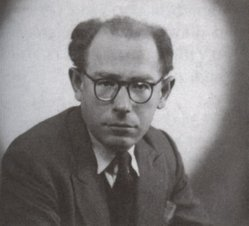
\includegraphics[width=0.6\linewidth]{Robinson}
		\caption{Abraham Robinson}
	\end{subfigure}
	\begin{subfigure}{0.4\textwidth}
		\centering
		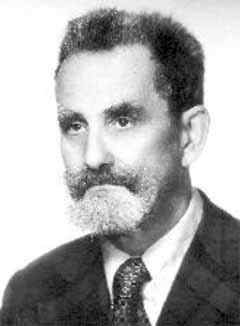
\includegraphics[width=0.4\linewidth]{Los}
		\caption{Jerzy \L o\'s}
	\end{subfigure}
\end{figure}
\end{frame}

\begin{frame}{Basic Idea}
\begin{itemize}
\setlength{\itemsep}{8pt}
	\item We construct a set of \textit{hyperreals}, denoted $\hreals$.
	\item $\hreals$ includes $\reals$, along with (a lot of) hyperreals.
	\item We construct a language of mathematical logic, using symbols like $\neg$, $\land$, $\lor$, $\forall$, etc.
	\item We show that any sentence of that language is true in $\reals$ iff it is true in $\hreals$ (transfer principle).
	\item We use transfer to prove things about $\reals$.
\end{itemize}
\end{frame}

\begin{frame}{Constructing $\hreals$}
\begin{itemize}
\setlength{\itemsep}{8pt}
	\item We start with the ring $\reals^\infty$.
	\item Identify sequences that are the same ``almost everywhere,'' like $\langle 0, 1, 1, \ldots \rangle \sim \langle 1, 1, 1, \ldots \rangle$.
	\item Sequences are the same almost everywhere if the set of indices at which they are the same is ``big.''
	\item The set of ``big'' sets of natural numbers is an \textit{ultrafilter} $\mathcal{F} \subseteq \mathcal{P}(\mathbb{N})$.
\end{itemize}
\end{frame}

\begin{frame}{Constructing $\hreals$}
\begin{itemize}
\setlength{\itemsep}{8pt}

\item Now we can define our equivalence relation $\sim$ by saying that $\langle r_1, r_2, r_3, \ldots \rangle \sim \langle s_1, s_2, s_3, \ldots \rangle$ iff $\{n \in \nats \sthat r_n = s_n \} \in \mathcal{F}$.

\item Write the equivalence class $[\langle r_1, r_2, r_3, \ldots \rangle]$.

\item Define $\hreals$ as the quotient ring of $\reals^\infty$ under $\sim$, i.e. $\hreals = \{[\langle r_1, r_2, r_3, \ldots \rangle] \sthat \langle r_1, r_2, \ldots \rangle \in \reals^\infty\}$.

\item Extend any function $f: \reals \to \reals$ to a new $\hr{f}: \hreals \to \hreals$.

$\hr{f}([\langle r_1, r_2, r_3, \ldots \rangle]) = [\langle f(r_1), f(r_2), f(r_3), \ldots \rangle]$.

\item We can also extend relations, like ``$\leq$.'' 

$\langle r_1, r_2, r_3, \ldots \rangle \leq \langle s_1, s_2, s_3, \ldots \rangle$ iff $\{n \in \nats \sthat r_n \leq s_n\} \in \mathcal{F}$.

\item For any $x \in \reals$, we can take $x \in \hreals$ to mean $[\langle x, x, x, \ldots \rangle]$.
\end{itemize}
\end{frame}

\begin{frame}{Transfer Principle}
\begin{itemize}
\setlength{\itemsep}{8pt}
\item Our language is made up of:
	\begin{itemize}
	\item logical connectives $\land$, $\lor$, $\to$, $\leftrightarrow$, and $\neg$,
	\item quantifiers $\forall$, $\exists$,
	\item parenthesis $($ and $)$,
	\item variables $x, y, z, \ldots$, and
	\item symbols for every element of $\reals$, every relation on $\reals$, and every function on $\reals$.
	\end{itemize}
\item Sentences are defined recursively. 

$(\forall x \in \reals)(x < x + 1)$ vs. $))5+\leq v_1 \leftrightarrow \neg \land 64$
\item If $\varphi$ is a sentence that ``talks about'' $\reals$, we can obtain $\hr{\varphi}$ by replacing each function and relation with its extension in $\hreals$.
\item \textbf{Transfer Principle:} Any sentence $\varphi$ is true iff $\hr{\varphi}$ is true.
\end{itemize}
\end{frame}

\begin{frame}{Structure of $\hreals$}
\begin{itemize}
\setlength{\itemsep}{10pt}
\item We call an element $x \in \hreals$:
	\begin{itemize}
	\item \textit{infinitesimal} if $|x| < r$ for any $r \in \reals^+$,
	\item \textit{unbounded} if $r < |x|$ for any $r \in \reals^+$, and
	\item \textit{appreciable} if it is neither infinitesimal nor unbounded.
	\end{itemize}
\item Arithmetic properties of hyperreals are mostly intuitive.
\item We say two elements $x, y \in \hreals$ are \textit{infinitely close}, and write $x \simeq y$, if $|x - y|$ is infinitesimal. $\simeq$ is an equivalence relation.
\item Any bounded hyperreal $x$ is infinitely close to a unique real number, called its \textit{standard part} and denoted $\stp{x}$.
\item $\st$ has most of the nice properties you'd like it to: $\stp{x + y} = \stp{x} + \stp{y}$, etc.
\end{itemize}
\end{frame}


\begin{frame}{Derivatives}
\begin{itemize}
\item Say $f: \reals \to \reals$. Extend $f$ to $\hr{f}: \hreals \to \hreals$
\item Fix $b \in \reals$. Let $\Delta x$ be infinitesimal, and let $\Delta f$ be $\hr{f}(b + \Delta x) - \hr{f}(b)$.
\item Then define $f'(b) = \stp{\frac{\Delta f}{\Delta x}}$. So $f'(b) \simeq \frac{\Delta f}{\Delta x}$
\item \textbf{Example:} Say $f(x) = x^2$. Then we have 
\begin{align*}
f'(3) &\simeq \frac{(3 + \Delta x)^2 - 3^2}{\Delta x} = \frac{9 + 6 \Delta x + (\Delta x)^2 - 9}{\Delta x} \\
	&= \frac{6 \Delta x + (\Delta x)^2}{\Delta x} = 6 + \Delta x \simeq 6
\end{align*}
\item So $f'(3) \simeq 6$. But these are both real numbers, so their difference is real. Hence $f'(3) = 6$.
\end{itemize}
\end{frame}

\begin{frame}{Proof: Chain Rule}
Let $f,g: \reals \to \reals$ be differentiable. Let $\Delta x$ be any nonzero infinitesimal, and $\Delta g = g(x + \Delta x) - g(x)$. Then
\begin{align*}
(f \circ g)'(x) &\simeq \frac{f(g(x + \Delta x)) - f(g(x))}{\Delta x}  \\
	&= \frac{f(g(x) + \Delta g) - f(g(x))}{\Delta g} \cdot \frac{\Delta g}{\Delta x} \\ 
	&\simeq f'(g(x))\cdot g'(x)
\end{align*}
So $(f \circ g)'(x) \simeq f'(g(x)) \cdot g'(x)$. But since both of these numbers are real, they must be identical.
\vspace{2mm}

When $\Delta g = 0$, $f(g(x) + \Delta g) - f(g(x)) = 0$ and so $(f \circ g)'(x) = 0$. 
\vspace{1mm}

Further, $g'(x) = \stp{\frac{\Delta g}{\Delta x}} = 0$, so $f'(g(x)) \cdot g'(x) = 0$.
\end{frame}



\end{document}